\documentclass[12pt,a4paper]{article}

\usepackage[utf8]{inputenc}
\usepackage[T1]{fontenc}
\usepackage[english]{babel}
\usepackage{graphicx}
\usepackage{float}
\usepackage{hyperref}
\usepackage{booktabs}
\usepackage{array}
\usepackage{geometry}
\usepackage{amsmath}
\usepackage{amssymb}
\usepackage{xcolor}
\usepackage{longtable}
\usepackage{enumitem}
\usepackage{tikz}
\usetikzlibrary{shapes.geometric, arrows.meta, positioning, fit, backgrounds}

\geometry{left=2.5cm,right=2.5cm,top=3cm,bottom=3cm}

\hypersetup{
    colorlinks=true,
    linkcolor=blue,
    urlcolor=blue,
    citecolor=black
}

\title{Project Management and Enhanced Design Document\\[0.3cm]
\large Workshop 3: Robust Design, Quality, Risk, and Operational Planning}
\author{
Omar Yesid Fonseca López \\
Daniel Felipe Barrera Suárez \\
Daniel Mateo Ballesteros Molina \\
Dania Lizeth Guzmán Triviño
}
\date{Bogotá, Colombia -- 2026}

\begin{document}

\begin{titlepage}
    \centering
    \vspace*{1cm}
    {\Large \textbf{Universidad Distrital Francisco José de Caldas}} \\
    \vspace{0.4cm}
    {\large Faculty of Engineering \\ Systems Engineering Program} \\
    \vspace{2.5cm}
    {\Huge \textbf{Project Management and Enhanced Design Document}} \\
    \vspace{0.5cm}
    {\Large \textbf{Workshop 3: Robust Design, Quality, Risk, and Operational Planning}} \\
    \vspace{2cm}
    \textbf{Authors (Engineering Team):} \\
    Omar Yesid Fonseca López (\texttt{oyfonsecal@udistrital.edu.co}) \\
    Daniel Felipe Barrera Suárez (\texttt{dfbarreras@udistrital.edu.co}) \\
    Daniel Mateo Ballesteros Molina (\texttt{dmballesterosm@udistrital.edu.co}) \\
    Dania Lizeth Guzmán Triviño (\texttt{dlguzmant@udistrital.edu.co}) \\
    \vfill
    \textbf{Course:} Systems Analysis \& Design \\
    \textbf{Professor:} Eng. Carlos Andrés Sierra, M.Sc. \\
    \vspace{1cm}
    Bogotá, Colombia \\
    2026
\end{titlepage}

\pagenumbering{roman}

\begin{abstract}
This document presents the consolidation of \textbf{Workshop 3} for the \textbf{Smart Campus Energy Management System} project at Sabio Caldas Campus. Building upon the systems analysis conducted in Workshop 1 and the preliminary design developed in Workshop 2, this document formulates a robust design proposal focused on technical feasibility, software quality, risk mitigation, and preparation for a controlled pilot implementation. The system adopts a distributed user-space architecture with autonomous agents capable of collecting telemetry, detecting inactivity, executing energy-saving policies, and operating with fault tolerance through local persistence and deferred synchronization.

In addition to architectural strengthening, this document incorporates a project management structure including a project charter, role definitions, schedule, resource plan, communication and control plan, implementation strategy, training plan, and continuous improvement framework. All of this demonstrates that the solution not only addresses the identified problem of energy waste in university laboratories but is also sufficiently structured to advance toward a measurable, controlled Proof of Concept aligned with good engineering and management practices.

The complete project repository is available at: \url{https://github.com/yecop/Systems-Analysis-and-Design}
\end{abstract}

\newpage
\tableofcontents
\newpage
\listoffigures
\newpage
\listoftables
\newpage

\pagenumbering{arabic}

\section{Executive Summary}
This document synthesizes the evolution of a system aimed at reducing energy waste in the laboratories of Sabio Caldas Campus, particularly in scenarios where equipment and peripherals remain powered on despite the absence of users. In \textit{Workshop 1}, the problem was identified from a systemic perspective, recognizing human, technical, and organizational factors. In \textit{Workshop 2}, a software-based solution was proposed that avoided dependencies on unauthorized IoT infrastructure. In this \textit{Workshop 3}, the proposal is strengthened through principles of robustness, quality control, risk management, and project planning.

The current proposal relies on local agents capable of monitoring activity, applying safe suspension rules, and reporting information to a database and visualization layer. Given the institutional environment's network restrictions, contingency mechanisms such as encrypted local storage and deferred synchronization are incorporated. Quality criteria, metrics, validation plans, and a pilot implementation roadmap are also defined, transforming the project from a technical idea into a more structured initiative prepared for gradual and controlled execution.

\section{Project Charter}

\subsection{Project Purpose}
The purpose of this project is to design, develop, and validate a Proof of Concept (PoC) for an intelligent energy management system that reduces unnecessary consumption in university laboratories by automating suspension actions and monitoring computer equipment activity. The system seeks to demonstrate that it is possible to improve campus energy efficiency without requiring deep changes to physical infrastructure or installation of additional network devices.

\subsection{Project Scope}
The scope includes robust architecture design, implementation of an autonomous Python agent, incorporation of fault tolerance mechanisms, quality testing, and a controlled pilot implementation on a reduced set of equipment. It also includes telemetry capture, local and remote event storage, and construction of an analytical dashboard to visualize preliminary energy savings results.

Large-scale institutionalization, acquisition of new physical infrastructure, and official integration with all university administrative systems are not within scope. The project is limited to an academic and technical Proof of Concept that allows feasibility and performance evaluation.

\subsection{Project Objectives}
\begin{itemize}[leftmargin=1.2cm]
    \item Design a robust software architecture that operates within institutional network and security restrictions.
    \item Implement an agent capable of detecting inactivity and executing energy-saving policies safely.
    \item Mitigate technical and operational risks through local persistence mechanisms, load validation, and deferred synchronization.
    \item Validate the solution through a controlled pilot with a set of technical and operational metrics.
    \item Produce evidence of feasibility for future scaling phases within the institution.
\end{itemize}

\subsection{Project Stakeholders}
The main project stakeholders include student users of the laboratories, faculty members responsible for the rooms, the engineering team designing and implementing the solution, technical support staff, campus administration interested in energy efficiency and security, and the course that frames the academic development of the project. Each of these actors has different interests: usability, operational continuity, energy savings, ease of maintenance, risk control, and solution quality.

\subsection{Success Criteria}
The project will be considered successful if the pilot demonstrates that the agent can adequately detect inactivity periods, execute energy-saving actions without affecting critical academic activities, maintain record integrity even during network failures, and produce sufficient data for impact analysis. Additionally, success will be measured by documentation clarity, design maintainability, and the possibility of future system expansion.

\section{System Evolution and Lessons Learned}

\subsection{Synthesis of Workshop 1}
In the first phase, a comprehensive analysis of the real system was conducted, identifying energy waste as a recurrent problem associated with university laboratory usage. A significant portion of consumption was observed not to be due exclusively to hardware deficiencies, but rather to usage practices such as leaving peripherals on, maintaining inactive sessions for long periods, or failing to perform timely shutdowns at the end of academic activities.

\subsection{Synthesis of Workshop 2}
In the second phase, a conceptual architecture oriented toward solving the problem through software was proposed. Approaches based on IoT devices or intensive centralized control were discarded due to institutional restrictions related to network, permissions, and deployment. As a result, a solution based on local agents operating in user space, interacting with operating system APIs, and reporting relevant events to external services was chosen.

\subsection{Improvements Introduced in Workshop 3}
In this stage, the design is refined from a robustness perspective. Fault tolerance mechanisms, quality assurance criteria, acceptance metrics, risk categorization, and a formal implementation structure are added. It is also recognized that a technical solution is insufficient without adequate project management, so schedule, resources, communications, control, and deployment preparation are incorporated.

\subsection{Risks Identified and Mitigated}
The main lesson is that an apparently simple solution can be strongly conditioned by the organizational and technical context. It was also learned that reliability in real environments requires considering contingencies from the design stage, especially when there are network blocks, variability in computational load, and sensitivity regarding potential loss of academic work. Finally, it became evident that documentation and traceability between phases strengthen project coherence and facilitate evaluation.

\section{Robust System Architecture}

\subsection{Architecture Overview}
The proposed architecture is decentralized and relies on an autonomous agent installed on each workstation participating in the pilot. This agent monitors user activity events, queries system status, and decides whether or not to apply a suspension or energy-saving policy. Generated records are ideally stored in a remote database; however, when connectivity is unavailable, a backup mechanism temporarily persists information locally.

\subsection{Quality Attributes Mapping}
System robustness is structured around several quality attributes. \textbf{Reliability} is supported by local persistence and deferred synchronization; \textbf{maintainability} is favored through modular component organization and separation between capture, decision, persistence, and communication; \textbf{scalability} is contemplated by allowing agents to be replicated across multiple equipment with minimal dependencies between them; \textbf{security} is addressed through encryption of local files and control of transmission paths; and \textbf{usability} is protected by avoiding suspensions when there are indications of relevant computational activity, even without direct mouse or keyboard interaction.

\subsection{Integration and Interfaces}
The system contemplates several main interfaces. First, a local interface with the operating system and monitoring libraries to identify activity events, peripheral status, and processor load. Second, a communication interface with external services, used to register events or send alerts. Third, an analytics interface to consume consolidated data and present it on a dashboard. These interfaces must operate under low coupling criteria, exception handling, and error traceability.

\subsection{Fault-Tolerant Architecture}
The robustified design proposes that the agent operates through independent modules or threads. If the communication channel with the cloud fails, the system must not stop or lose critical information; instead, it must locally store telemetry and suspension events in an encrypted CSV file. When network connectivity is restored, the system must synchronize pending data with the remote database. This reduces vulnerability to firewall blocks, temporary failures of external services, or communication channel interruptions.

\begin{figure}[H]
\centering
\resizebox{0.92\textwidth}{!}{%
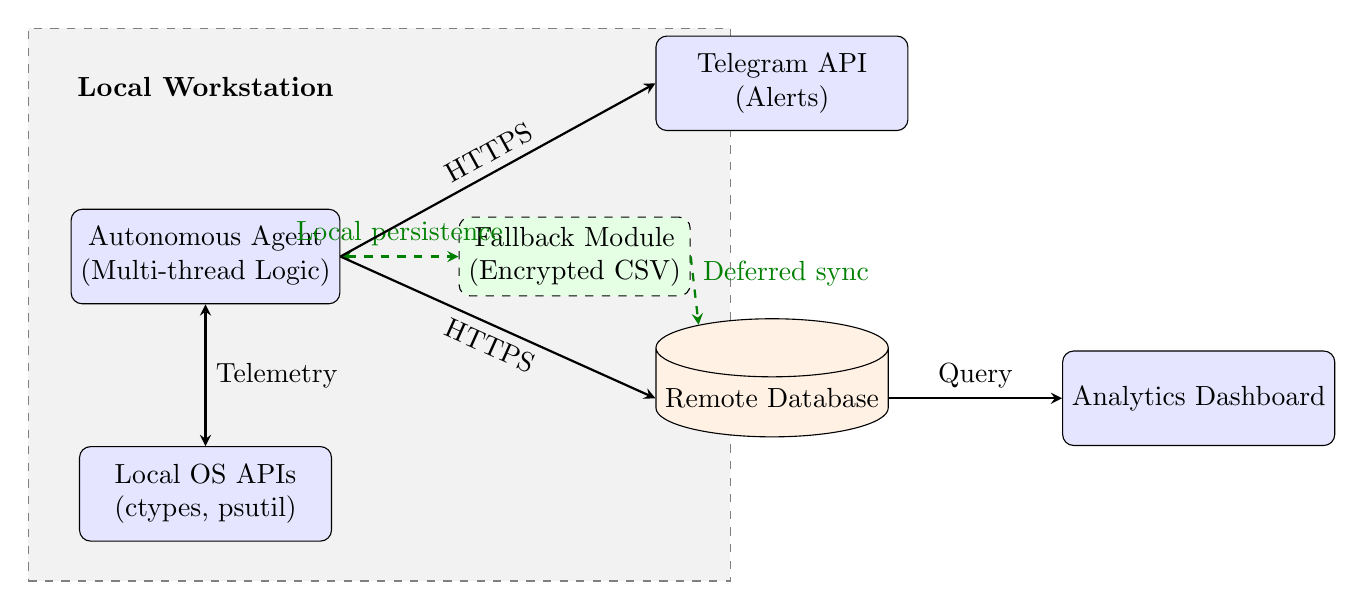
\begin{tikzpicture}[
    node distance=2cm and 3cm,
    box/.style={draw, rectangle, minimum width=3.2cm, minimum height=1.2cm, align=center, fill=blue!10, rounded corners},
    db/.style={draw, cylinder, shape border rotate=90, aspect=0.25, minimum height=1.5cm, minimum width=2.4cm, align=center, fill=orange!10},
    robust/.style={draw, rectangle, minimum width=2.8cm, minimum height=1cm, align=center, fill=green!10, rounded corners, dashed},
    arrow/.style={->, >=stealth, thick}
]

\node[box] (agent) {Autonomous Agent\\(Multi-thread Logic)};
\node[box, below=1.8cm of agent] (os) {Local OS APIs\\(ctypes, psutil)};
\node[robust, right=1.5cm of agent] (fallback) {Fallback Module\\(Encrypted CSV)};
\node[above=1.3cm of agent] (title) {\textbf{Local Workstation}};

\begin{scope}[on background layer]
    \node[fill=gray!10, draw=gray, dashed, fit=(title) (agent) (os) (fallback), inner sep=0.5cm] {};
\end{scope}

\node[box, right=4cm of agent, yshift=2.2cm] (telegram) {Telegram API\\(Alerts)};
\node[db, right=4cm of agent, yshift=-1.8cm] (mysql) {Remote Database};
\node[box, right=2.2cm of mysql] (powerbi) {Analytics Dashboard};

\draw[arrow, <->] (agent) -- node[right] {Telemetry} (os);
\draw[arrow, <->, dashed, color=green!50!black] (agent) -- node[above] {Local persistence} (fallback);
\draw[arrow] (agent.east) -- node[above, sloped] {HTTPS} (telegram.west);
\draw[arrow] (agent.east) -- node[below, sloped] {HTTPS} (mysql.west);
\draw[arrow, dashed, color=green!50!black] (fallback.east) -- node[right, near start] {Deferred sync} (mysql.north west);
\draw[arrow] (mysql.east) -- node[above] {Query} (powerbi.west);

\end{tikzpicture}%
}
\caption{Decentralized robust architecture with fault tolerance and local persistence}
\label{fig:robust_architecture}
\end{figure}

\section{Risk Management Plan}

\subsection{Risk Identification}
A systematic risk identification was conducted considering technical, operational, security, and project management dimensions. The objective is to anticipate scenarios that could compromise system functionality, pilot continuity, or the quality of collected evidence.

\subsection{Risk Categories}
Technical risks include communication failures, agent logic errors, and unexpected operating system behavior. Operational risks encompass inadequate user usage, rejection of automation, or lack of timely access to laboratories. Security risks include exposure of sensitive telemetry information or unauthorized execution. Finally, project management risks comprise delays, excessive dependence on certain team members, limited time availability, and coordination difficulties.

\subsection{Risk Matrix and Mitigation Strategies}
\begin{table}[H]
\caption{Project risk management matrix}
\label{tab:risks}
\centering
\begin{tabular}{|p{0.9cm}|p{4.2cm}|p{1.8cm}|p{1.8cm}|p{5.5cm}|}
\hline
\textbf{ID} & \textbf{Risk} & \textbf{Prob.} & \textbf{Impact} & \textbf{Mitigation Strategy} \\
\hline
R-01 & HTTPS requests blocked by institutional firewall & High & Medium & Local encrypted CSV persistence and deferred synchronization when network becomes available. \\
\hline
R-02 & False positive inactivity during heavy CPU tasks & Medium & Critical & CPU load verification before suspension; if load exceeds threshold, reset inactivity counter. \\
\hline
R-03 & External alert service outage or unavailability & Low & Low & Structured exception handling and prioritization of local logic over external notifications. \\
\hline
R-04 & Loss or corruption of local backup data & Low & High & Encryption, write validation, error handling, and periodic synchronization. \\
\hline
R-05 & User resistance to automation & Medium & Medium & Prior communication, controlled pilot, explanation of purpose, and feedback collection. \\
\hline
R-06 & Delays due to academic workload or dependency on few members & Medium & Medium & Clear responsibility distribution, weekly follow-up, and milestone-based progress review. \\
\hline
\end{tabular}
\end{table}

\begin{figure}[H]
\centering
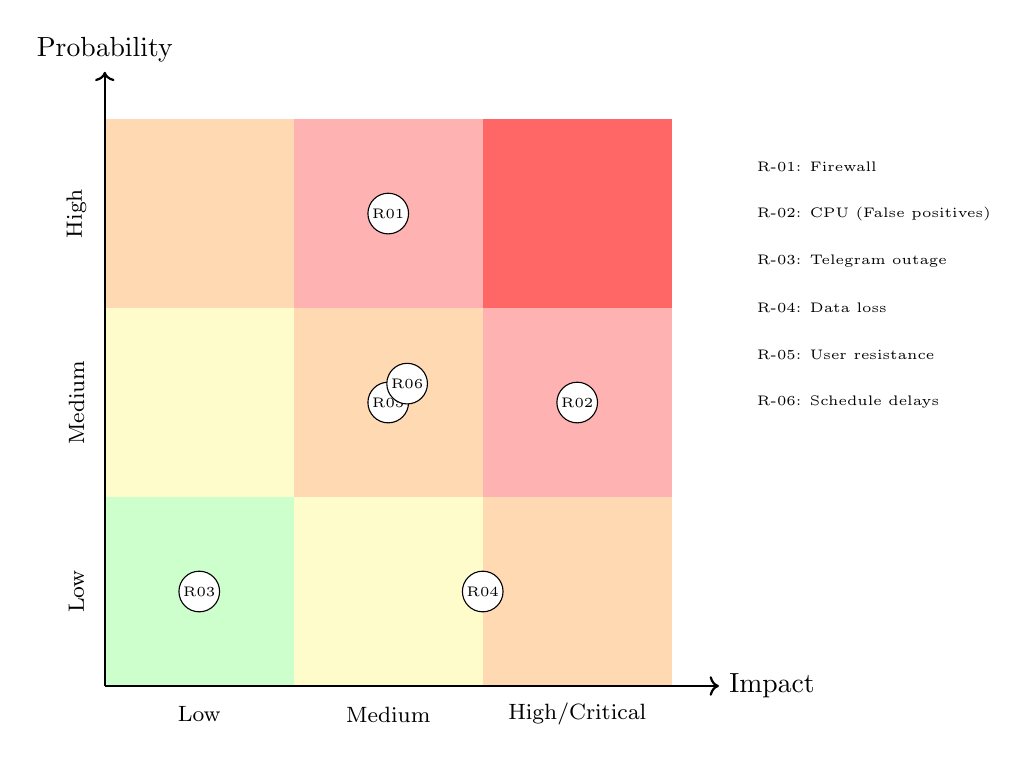
\begin{tikzpicture}[scale=1.2]
    % Heat grid (ISO 31000)
    \fill[green!20] (0,0) rectangle (2,2);
    \fill[yellow!20] (2,0) rectangle (4,2); \fill[yellow!20] (0,2) rectangle (2,4);
    \fill[orange!30] (4,0) rectangle (6,2); \fill[orange!30] (2,2) rectangle (4,4); \fill[orange!30] (0,4) rectangle (2,6);
    \fill[red!30] (4,2) rectangle (6,4); \fill[red!30] (2,4) rectangle (4,6);
    \fill[red!60] (4,4) rectangle (6,6);

    % Axes
    \draw[thick, ->] (0,0) -- (6.5,0) node[right] {Impact};
    \draw[thick, ->] (0,0) -- (0,6.5) node[above] {Probability};

    % Labels
    \node at (1,-0.3) {\footnotesize Low}; \node at (3,-0.3) {\footnotesize Medium}; \node at (5,-0.3) {\footnotesize High/Critical};
    \node[rotate=90] at (-0.3,1) {\footnotesize Low}; \node[rotate=90] at (-0.3,3) {\footnotesize Medium}; \node[rotate=90] at (-0.3,5) {\footnotesize High};

    % Risks
    \node[draw, circle, fill=white, inner sep=1pt] at (3,5) {\tiny R01};
    \node[draw, circle, fill=white, inner sep=1pt] at (5,3) {\tiny R02};
    \node[draw, circle, fill=white, inner sep=1pt] at (1,1) {\tiny R03};
    \node[draw, circle, fill=white, inner sep=1pt] at (4,1) {\tiny R04};
    \node[draw, circle, fill=white, inner sep=1pt] at (3,3) {\tiny R05};
    \node[draw, circle, fill=white, inner sep=1pt] at (3.2,3.2) {\tiny R06};

    % Legend
    \node[anchor=west, font=\tiny] at (6.8,5.5) {R-01: Firewall};
    \node[anchor=west, font=\tiny] at (6.8,5.0) {R-02: CPU (False positives)};
    \node[anchor=west, font=\tiny] at (6.8,4.5) {R-03: Telegram outage};
    \node[anchor=west, font=\tiny] at (6.8,4.0) {R-04: Data loss};
    \node[anchor=west, font=\tiny] at (6.8,3.5) {R-05: User resistance};
    \node[anchor=west, font=\tiny] at (6.8,3.0) {R-06: Schedule delays};
\end{tikzpicture}
\caption{Matrix visualization of risk impact and probability}
\label{fig:risk_matrix}
\end{figure}

\subsection{Risk Monitoring and Control}
During the pilot, periodic monitoring of prioritized risks will be conducted. A weekly review of incident status, synchronization failures, agent behavior, and milestone compliance will be established. The quality and management lead will review collected evidence, classify events, and propose adjustments when recurrent error patterns are detected.

\subsection{Contingency Plans}
In case of network failures, local persistence will be activated; for erroneous inactivity detections, the decision threshold will be temporarily raised while parameters are adjusted; in case of user rejection, the pilot will be limited to clearly authorized equipment; and for schedule delays, critical deliverables will be prioritized: stable agent, test evidence, and results consolidation.

\section{Quality Assurance Framework}

\subsection{Quality Objectives}
The system must meet minimum objectives of functional correctness, operational reliability, fault recovery capability, maintainability, and suitability for the university context. Agent behavior must be predictable, auditable, and sufficiently flexible to adapt to different workloads without negatively affecting user experience.

\subsection{Quality Metrics}
The following metrics are proposed: rate of correct suspensions relative to total detected events; false positive inactivity rate; percentage of events stored without loss; average deferred data synchronization time; number of incidents per communication failure; and basic test coverage of critical modules. These metrics will allow measurement of both technical performance and operational stability.

\subsection{Validation Methods}
Validation will rely on unit tests, integration tests, computational stress tests, and controlled observation during the pilot. Unit tests will verify timing and inactivity logic; integration tests will evaluate persistence, reading, writing, and synchronization; stress tests will verify system response under heavy processes; and laboratory observations will identify discrepancies between expected design and real behavior.

\subsection{Acceptance Criteria}
Acceptance criteria will establish that the system must not suspend equipment during high computational load processes, maintain a high percentage of record retention even during network failures, exhibit reproducible behavior across all pilot equipment, and ensure the final dashboard receives consistent data for analysis. If minor failures occur, they will be evaluated to determine whether they compromise the main purpose of the Proof of Concept.

\subsection{QA Flow}
The quality assurance flow will follow a sequence of test case preparation, technical execution, findings registration, correction, revalidation, and approval for the next environment. This dynamic will ensure that the transition from alpha to beta phase is supported by evidence rather than mere perception of functionality.

\begin{figure}[H]
\centering
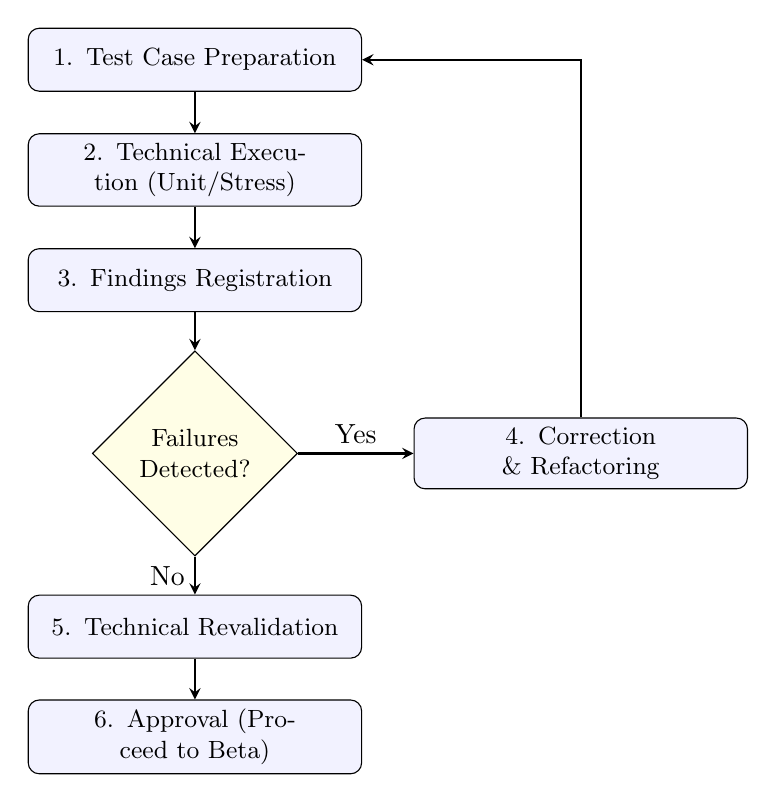
\begin{tikzpicture}[
    node distance=1.4cm,
    block/.style={rectangle, draw, fill=blue!5, text width=4cm, text centered, rounded corners, minimum height=0.8cm, font=\small},
    decision/.style={diamond, draw, fill=yellow!10, text width=2cm, text centered, inner sep=0pt, font=\small},
    arrow/.style={thick, ->, >=stealth}
]
    \node (prep) [block] {1. Test Case Preparation};
    \node (exec) [block, below of=prep] {2. Technical Execution (Unit/Stress)};
    \node (reg) [block, below of=exec] {3. Findings Registration};
    \node (check) [decision, below of=reg, yshift=-0.8cm] {Failures Detected?};
    \node (fix) [block, right of=check, xshift=3.5cm] {4. Correction \& Refactoring};
    \node (val) [block, below of=check, yshift=-0.8cm] {5. Technical Revalidation};
    \node (app) [block, below of=val] {6. Approval (Proceed to Beta)};

    \draw [arrow] (prep) -- (exec);
    \draw [arrow] (exec) -- (reg);
    \draw [arrow] (reg) -- (check);
    \draw [arrow] (check) -- node[anchor=south] {Yes} (fix);
    \draw [arrow] (fix) |- (prep);
    \draw [arrow] (check) -- node[anchor=east] {No} (val);
    \draw [arrow] (val) -- (app);
\end{tikzpicture}
\caption{Iterative Quality Assurance process flow}
\label{fig:qa_flow}
\end{figure}

\section{Project Management Plan}

\subsection{Team Structure and Roles}
Team organization responds to a functional distribution aimed at ensuring technical and operational coverage of the project.

\begin{table}[H]
\caption{Team roles and responsibilities}
\label{tab:roles}
\centering
\begin{tabular}{|p{3cm}|p{4.8cm}|p{6cm}|}
\hline
\textbf{Team Member} & \textbf{Role} & \textbf{Key Responsibilities} \\
\hline
Omar Yesid Fonseca López & Project Manager \& QA Lead & Schedule tracking, risk management, general coordination, and quality validation. \\
\hline
Daniel Felipe Barrera Suárez & Systems Architect & Robust architecture design, module integration, and structural decisions. \\
\hline
Daniel Mateo Ballesteros Molina & Algorithms \& Agent Specialist & Agent implementation, monitoring logic, load validation, and local persistence. \\
\hline
Dania Lizeth Guzmán Triviño & Analytics \& Communications & Data consolidation, dashboard, documentation support, and project communication strategy. \\
\hline
\end{tabular}
\end{table}

\subsection{Project Schedule}
A six-week execution period is proposed for the Proof of Concept, with defined milestones for development, testing, pilot, and consolidation.

\begin{table}[H]
\caption{General project schedule}
\label{tab:schedule}
\centering
\begin{tabular}{|p{4.2cm}|p{1.1cm}|p{1.1cm}|p{1.1cm}|p{1.1cm}|p{1.1cm}|p{1.1cm}|}
\hline
\textbf{Activity} & \textbf{W1} & \textbf{W2} & \textbf{W3} & \textbf{W4} & \textbf{W5} & \textbf{W6} \\
\hline
Architecture adjustment and robust design & X & X &  &  &  &  \\
\hline
Agent and fallback implementation & X & X & X &  &  &  \\
\hline
Internal testing and quality assurance &  &  & X & X &  &  \\
\hline
Pilot deployment in laboratory &  &  &  & X & X &  \\
\hline
Data consolidation and dashboard &  &  &  &  & X & X \\
\hline
Documentation closure and final evaluation &  &  &  &  &  & X \\
\hline
\end{tabular}
\end{table}

\begin{figure}[H]
\centering
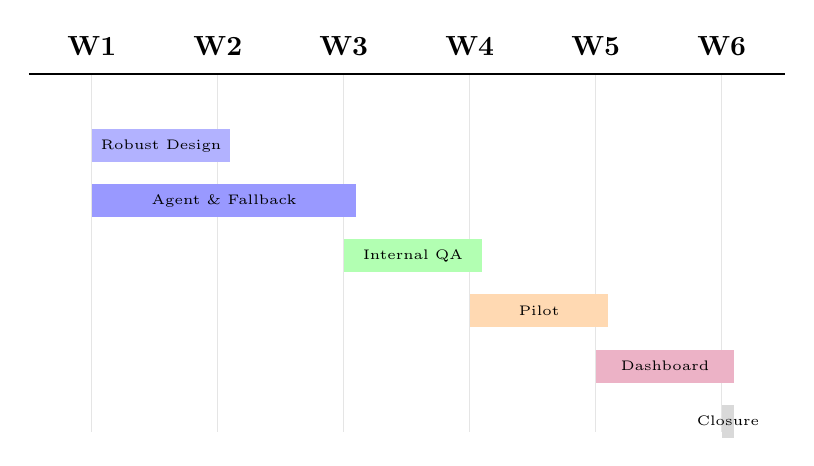
\begin{tikzpicture}[xscale=1.6, yscale=0.7]
    % Weeks
    \foreach \s in {1,...,6} {
        \node at (\s, 0.5) {\textbf{W\s}};
        \draw[gray!20] (\s, 0) -- (\s, -6.5);
    }
    
    % Tasks
    \fill[blue!30] (1, -1) rectangle (2.1, -1.6) node[midway, black, font=\tiny] {Robust Design};
    \fill[blue!40] (1, -2) rectangle (3.1, -2.6) node[midway, black, font=\tiny] {Agent \& Fallback};
    \fill[green!30] (3, -3) rectangle (4.1, -3.6) node[midway, black, font=\tiny] {Internal QA};
    \fill[orange!30] (4, -4) rectangle (5.1, -4.6) node[midway, black, font=\tiny] {Pilot};
    \fill[purple!30] (5, -5) rectangle (6.1, -5.6) node[midway, black, font=\tiny] {Dashboard};
    \fill[gray!30] (6, -6) rectangle (6.1, -6.6) node[midway, black, font=\tiny] {Closure};

    \draw[thick] (0.5,0) -- (6.5,0);
\end{tikzpicture}
\caption{Visual timeline of the Proof of Concept (6 weeks)}
\label{fig:timeline}
\end{figure}

\subsection{Milestones, Deliverables, Dependencies, and Critical Path}
The main milestones are: completion of robust design, implementation of stable agent, approval of internal tests, pilot deployment, dashboard consolidation, and documentation closure. Associated deliverables include agent code, risk matrix, QA results, telemetry records, and technical report. The critical path depends especially on agent stability and successful completion of the internal testing phase, as failure in this stage would directly impact pilot initiation.

\subsection{Resource Plan}
The project primarily requires human and software resources. No significant investment in additional hardware is planned since the solution runs on existing equipment. Python and local monitoring libraries, CSV storage for contingency, a remote database for consolidation, and a visualization tool for the dashboard will be used. Team capacity is estimated at partial weekly dedication over six weeks, focused on development, testing, documentation, and results analysis.

\subsection{Budget and Resource Plan}
Given the software-defined nature of this Proof of Concept, no additional hardware procurement is required. The operational cost is based on the engineering team's time allocation (4 engineers × 20 hours/week × 6 weeks). All software tools used are open-source or have free tiers, making the PoC highly cost-effective and scalable for institutional adoption.

\begin{table}[H]
\caption{Budget estimation for the PoC execution}
\centering
\begin{tabular}{|p{5cm}|p{3cm}|p{3cm}|p{2.5cm}|}
\hline
\textbf{Resource} & \textbf{Type} & \textbf{Cost} & \textbf{Notes} \\
\hline
Engineering team (4×20h×6 weeks) & Human & \$0 (academic) & Course project effort \\
\hline
Cloud database (MySQL DBaaS) & Software & \$0 & Free tier (e.g., Clever Cloud, Aiven) \\
\hline
Telegram Bot API & Software & \$0 & Free for PoC scale \\
\hline
Power BI / Looker Studio & Software & \$0 & Free tier available \\
\hline
Python libraries (psutil, requests, cryptography) & Software & \$0 & Open source \\
\hline
GitHub repository & Infrastructure & \$0 & Student pack / free \\
\hline
\textbf{Total estimated cost} & & \multicolumn{2}{|c|}{\textbf{\$0 USD (academic PoC)}} \\
\hline
\end{tabular}
\label{tab:budget}
\end{table}

\subsection{Communication and Control Plan}
Weekly internal meetings will be established to review progress, risks, and blockers. Each team member will report the status of their tasks and relevant findings. For external stakeholders, especially laboratory faculty or supervisors, brief communications will be prepared prior to the pilot indicating purpose, scope, involved equipment, and precautionary measures. Project control will be carried out through milestone tracking, deliverable review, and periodic validation of risk and quality status.

\section{Implementation and Readiness Strategy}

\subsection{Deployment Strategy}
Implementation will follow a gradual approach. First, an alpha phase will be executed on the team's own equipment to validate basic agent behavior. Then, a beta phase will proceed on a small set of laboratory computers with prior authorization. Finally, data consolidation and pilot results analysis will be performed.

\begin{table}[H]
\caption{Pilot implementation phases}
\label{tab:implementation}
\centering
\begin{tabular}{|p{2cm}|p{2cm}|p{6cm}|p{4.3cm}|}
\hline
\textbf{Phase} & \textbf{Scope} & \textbf{Main Activities} & \textbf{Acceptance Criteria} \\
\hline
Alpha & 4 team member laptops & Logic verification, internal testing, fallback validation, log review. & Stable operation without improper suspensions. \\
\hline
Beta & 5 laboratory computers & Controlled deployment, real observation, telemetry collection, parameter adjustment. & Useful evidence and consistent behavior in real environment. \\
\hline
Closure & Analytical consolidation & Synchronization, dashboard, preliminary savings and event analysis. & Integrated data ready for final evaluation. \\
\hline
\end{tabular}
\end{table}

\subsection{Infrastructure Requirements}
Access to authorized laboratory equipment, local execution permissions for the agent, eventual connectivity for data synchronization, and a remote database environment or central repository to store consolidated telemetry are required. A visualization tool is also needed to build the final pilot dashboard.

\subsection{Dependencies and Preconditions}
Pilot execution depends on authorization to intervene in a controlled set of equipment, availability of team members to conduct tests and monitoring, and correct agent configuration on each station. A procedure to extract or synchronize data in case of limited connectivity during the test is also necessary.

\subsection{Change Management}
Any modification to suspension logic, decision thresholds, or persistence format must be registered and justified. The goal is to avoid improvised changes during the pilot. Adjustments must be approved by the component lead and communicated to the rest of the team to maintain traceability and coherence between documentation, code, and results.

\subsection{Training Plan}
Before pilot deployment, team members must review the installation, execution, monitoring, and failure recovery procedures. Additionally, a brief explanation will be prepared for laboratory supervisors or involved users, emphasizing the pilot's purpose, expected effects, and channels for reporting incidents or concerns.

\subsection{User Adoption Strategy}
Although the pilot has limited scope, it is important to foster a positive perception of the solution. It will be explained that the system seeks to optimize resources without interfering with legitimate academic work. An approach of accompaniment and observation will be privileged over strict imposition, collecting feedback for future iterations.

\section{Continuous Improvement Strategy}

\subsection{Feedback Mechanisms}
Continuous improvement will rely on three main sources: technical test results, pilot observations, and comments from users or laboratory supervisors. Each of these sources will allow detection of necessary adjustments in thresholds, wait times, record formats, and system behavior in specific contexts.

\subsection{Adaptive Management}
The project assumes that some parameters will need calibration based on usage experience. Therefore, the architecture and documentation have been designed in a modular and adjustable manner, allowing improvements to be introduced without completely redesigning the solution. This adaptive capacity is especially valuable in a real environment with changing restrictions.

\subsection{Post-Implementation Metrics}
After the pilot, metrics such as number of suspension events, percentage of valid events, reported incidents, volume of data recovered through deferred synchronization, and basic perception of system utility will be evaluated. These metrics will allow assessment not only of whether the system works, but also whether it generates sufficient evidence to justify a subsequent expansion phase.

\section{Visual Representations and Tools}
This document incorporates diagrams and tables that facilitate understanding of the architecture, risks, and project planning. For an extended version of the work, it is recommended to complement with a formal Gantt chart, a matrix visualization of risk impact and probability, and a specific flow of the quality assurance process. Tools such as draw.io, Lucidchart, Microsoft Project, or TikZ can be used to improve visual presentation and project traceability.

\begin{figure}[H]
\centering
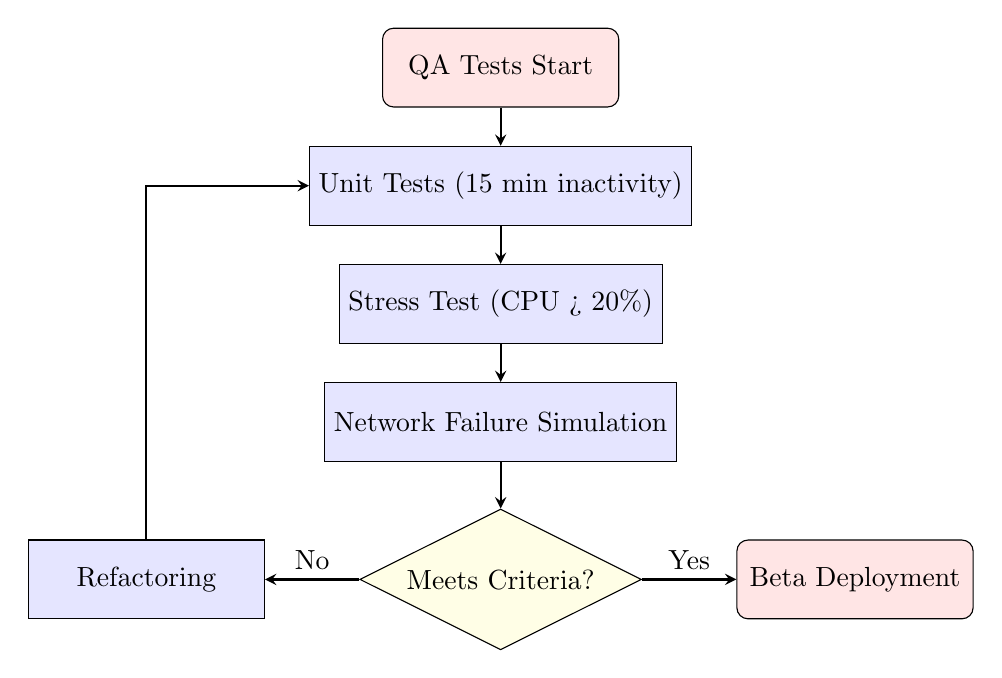
\begin{tikzpicture}[
    node distance=1.5cm,
    startstop/.style={rectangle, rounded corners, minimum width=3cm, minimum height=1cm, text centered, draw=black, fill=red!10},
    process/.style={rectangle, minimum width=3cm, minimum height=1cm, text centered, draw=black, fill=blue!10},
    decision/.style={diamond, aspect=2, minimum width=3cm, minimum height=1cm, text centered, draw=black, fill=yellow!10},
    arrow/.style={thick,->,>=stealth}
]
    \node (start) [startstop] {QA Tests Start};
    \node (unit) [process, below of=start] {Unit Tests (15 min inactivity)};
    \node (stress) [process, below of=unit] {Stress Test (CPU > 20\%)};
    \node (network) [process, below of=stress] {Network Failure Simulation};
    \node (dec1) [decision, below of=network, yshift=-0.5cm] {Meets Criteria?};
    \node (stop) [startstop, right of=dec1, xshift=3cm] {Beta Deployment};
    \node (fix) [process, left of=dec1, xshift=-3cm] {Refactoring};

    \draw [arrow] (start) -- (unit);
    \draw [arrow] (unit) -- (stress);
    \draw [arrow] (stress) -- (network);
    \draw [arrow] (network) -- (dec1);
    \draw [arrow] (dec1) -- node[anchor=south] {Yes} (stop);
    \draw [arrow] (dec1) -- node[anchor=south] {No} (fix);
    \draw [arrow] (fix) |- (unit);
\end{tikzpicture}
\caption{Quality Assurance and Testing Framework Flow}
\label{fig:qa_flow_detailed}
\end{figure}

\section{References}
\begin{enumerate}
    \item International Organization for Standardization. \textit{ISO 31000: Risk Management -- Guidelines}. ISO, 2018.
    \item International Organization for Standardization and International Electrotechnical Commission. \textit{ISO/IEC 25010: Systems and Software Quality Requirements and Evaluation (SQuaRE) -- System and Software Quality Models}. ISO/IEC, 2011.
    \item Project Management Institute. \textit{A Guide to the Project Management Body of Knowledge (PMBOK Guide)}. 7th ed., PMI, 2021.
    \item Carnegie Mellon University. \textit{CMMI for Development, Version 2.0}. CMMI Institute, 2018.
    \item Institute of Electrical and Electronics Engineers. \textit{IEEE Standard for Software Reviews and Audits}. IEEE.
    \item T. Hong, H. Taylor-Lange, S. D'Oca, D. Yan, and S. Corgnati, "Advances in research and applications of energy-related occupant behavior in buildings," \textit{Energy and Buildings}, vol. 116, pp. 694-702, 2016.
    \item C. A. Sierra, "Workshop No. 1: Systems Analysis," Systems Analysis \& Design Course, Universidad Distrital Francisco José de Caldas, 2026.
\end{enumerate}

\section{Appendices}

\subsection{Repository Structure and Deliverables}
The following files and folders are available in the project GitHub repository (\url{https://github.com/yecop/Systems-Analysis-and-Design}):

\begin{table}[H]
\caption{Repository structure and workshop deliverables}
\centering
\begin{tabular}{|p{3.5cm}|p{3cm}|p{6.5cm}|}
\hline
\textbf{Folder / File} & \textbf{Workshop} & \textbf{Description} \\
\hline
/docs/Workshop1\_Analysis.pdf & 1 & Final IEEE-formatted systems analysis document \\
\hline
/data/observacion\_directa.csv & 1 & Direct observation logs (occupancy vs. energy waste) \\
\hline
/data/luminosidad\_*.csv & 1 & Environmental lux meter correlation data (3 cases) \\
\hline
/data/Datos\_encuestas.csv & 1 & Raw structured survey responses (n=35) \\
\hline
/assets/diagrams/ & 1,2,3 & Architecture diagrams and visual representations \\
\hline
/docs/Workshop2\_Design.pdf & 2 & Software-defined energy management PoC design \\
\hline
/src/agent/ & 2,3 & Autonomous telemetry agent source code (Python) \\
\hline
/Workshop3\_Management/ & 3 & This document (PDF) and supporting management artifacts \\
\hline
/README.md & 1,2,3 & Project overview and navigation (updated) \\
\hline
\end{tabular}
\label{tab:repository}
\end{table}

\subsection{Quality Assurance Checklist}
The following checklist was used during the QA phase (referenced in Section 6):

\begin{itemize}
    \item Unit test: Idle detection accuracy (target: 100\% after 15 min of inactivity)
    \item Unit test: CPU load verification before suspension (threshold: $<$20\%)
    \item Integration test: Local CSV encryption and write validation
    \item Integration test: Fallback activation on network failure simulation
    \item Stress test: Video rendering benchmark (no false suspension during $>$20\% CPU)
    \item Network test: Deferred synchronization after connectivity restoration
\end{itemize}

\subsection{Detailed Risk Register}
Complete risk register extending Table~\ref{tab:risks}:

\begin{longtable}{|p{1cm}|p{3cm}|p{2cm}|p{2cm}|p{2cm}|p{2.5cm}|}
\hline
\textbf{ID} & \textbf{Risk} & \textbf{Prob.} & \textbf{Impact} & \textbf{Trigger} & \textbf{Contingency} \\
\hline
R-01 & Firewall blocks HTTPS requests & High & Medium & HTTP 403/Timeout & Local CSV fallback \\
\hline
R-02 & False positive on high CPU load & Medium & Critical & CPU $>$20\% for $>$5 min & Reset counter, log event \\
\hline
R-03 & Telegram API outage & Low & Low & API timeout & Skip notification, suspend anyway \\
\hline
R-04 & Local data corruption & Low & High & CSV checksum fails & Periodic backup, retry sync \\
\hline
R-05 & User resistance & Medium & Medium & User complaints & Pilot on authorized PCs only \\
\hline
R-06 & Schedule delays & Medium & Medium & Missed milestone & Prioritize critical path \\
\hline
\caption{Detailed risk register}
\label{tab:risk_register}
\end{longtable}

\subsection{Project Repository Link}
The complete project repository can be accessed at: \url{https://github.com/yecop/Systems-Analysis-and-Design}

All documentation, source code, datasets, and diagrams are available under an academic use license.

\end{document}